\section{Collaboration}
This project was used as a capstone project. It was given as one of various options that the team could choose for their capstone. The reason this specific project was chosen was because it was intriguing, since none of us had any previous experience in AI and could therefore learn something new and relevant to current industry trends.

For this project we had various people collaborating. The team consisted of 1 faculty advisor, 1 business mentor, 1 faculty mentor, SCORE 2021 prompt sponsor, and 4 undergrads. It was set up to where the business mentor would be the customer, since he already had industry experience. Since this is used as a capstone there are course assignments that needed to be completed this is where the faculty mentor was used for. He provided feedback to make sure the documentation for the project would satisfy course assignments. The faculty advisor assisted with AI components design questions, since he has a background in AI. He was able to provide insightful information on which possible implementations may be needed for the AI components. The prompt sponsor was used to clarify project requirements. One undergrad was assigned the role of team liaison for easier communication between the different people involved.

In the beginning the team was split into two parts AI and UI where the AI components were considered priority. Three undergrads focused on the three requirements needed for the AI which are epic to user story, user story optimization, user stories to tasks and the last one focused on the UI requirements of visualization of their relationships. Later into the project the UI was moved as top priority. The UI consisted of visualizations between the relationships, showing the user suggestions and integrating the new buttons to the Main UI. By breaking up the AI and UI into parts allowed for more efficiency. Each component the undergrads chose was based on what intrigued them the most.

The team met a minimum of 2 times per week to go over documentation that was needed to complete the course and work on implementing the AI components and UI for the project. These meetings would feed into the business mentor meetings that were held once a week. Each time a new implementation piece was completed, it was discussed during the business mentor meetings to receive feedback from a customer perspective.

\begin{figure*}
\centerline{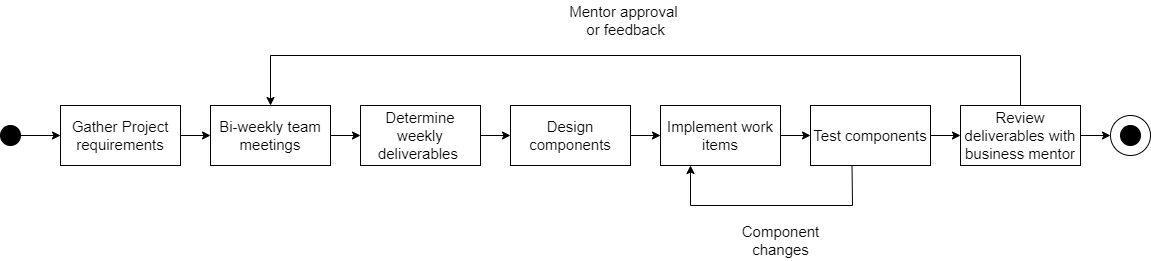
\includegraphics[width=\textwidth,height=\textheight,keepaspectratio]{./figure/ActivityDiagram.png}}
\caption{Activity Diagram outlining the development processes}
\label{fig:ExampleDataFlowDiagram}
\end{figure*}\

In the following sections, we will describe more in detail what work items and deliverables we performed during the project lifecycle.